\documentclass[10pt]{article}
\usepackage{slashbox}
\usepackage{spheric}
\usepackage{multirow}
%%%TITLE
\title{The study on SPH method with space variable smoothing length and its applications to multi-phase flow}
\date{}

%%AFFILIATIONS
\author[$\relax$]{Shi Wenkui}
\author[$\relax$]{Shen Yanming}
\author[$\relax$]{Chen Jianqiang$^\dagger$}

\affil[$\relax$]{China Aerodynamics Research and Development Center, Sichuan Mianyang 621000, China}

\affil[$\relax$]{\email{\dagger}{helloswk@126.com}}


%%DOCUMENT
\begin{document}

\maketitle

%\SelectedTopics{}

%%PLEASE PUT YOUR ABSTRACT HERE
\begin{abstract}
In the past, most studies about variable smoothing length were aimed to improve computation accuracy. Smoothing length is connected to density, varying with time. Besides, most of its applications were focused on astrophysics and detonations \cite{qiang2009numerical}.

This paper aims to improve the computational efficiency for solving multiphase flow by using space variable smoothing length, while the numerical accuracy is still held. Firstly, an initial particle diffusion distribution model is adopted. Then, in order to ensure the particle numbers in support domain for each particle almost unchanged, different particles are assigned to an independent smoothing lengths and masses. Meanwhile, some techniques are introduced to keep the symmetry of particle interactions.

Main results are presented in Figure \ref{fig:15}. In air bubble rising case, the bubble shapes and position at different times obtained by irregular particle distribution are consistent with those achieved by regular particle distribution. In addition, in asymmetric wedge water entry case, the impact acceleration computed by irregular particle distribution with variable smoothing length agrees well with that achieved by regular particle distribution. It's worth noting that the particle numbers of both cases are decreased by about 1/4 compared to regular particle distribution, and the computation times are reduced by 25\% (Table \ref{tab:15}). It indicates that this method is suitable to simulate the problems of complex engineering such as three-dimensional multi-phase flow and water impact.

\begin{figure}[!htb]
\centering
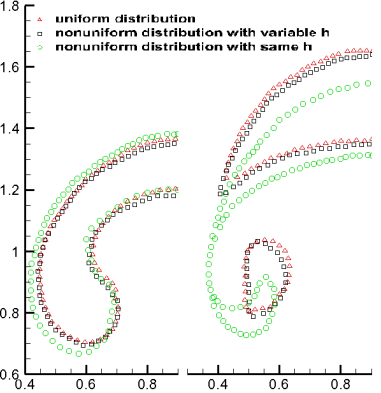
\includegraphics[width=0.35\textwidth]{15-11.png}~~
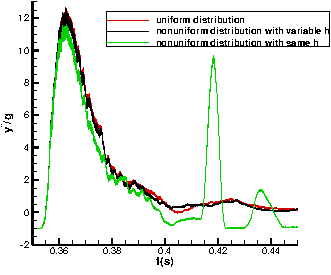
\includegraphics[width=0.45\textwidth]{15-12.pdf}
\caption{Left: Air bubble rising ($t\sqrt{g/R}=3.2,~4.8$); Right: Wedge water entry.}\label{fig:15}
\end{figure}

\begin{table}[!htb]
\centering
\caption{Comparison of computational efficiency}\label{tab:15}
\begin{tabular}{c|c|c|c|c}
\hline
\multirow{2}{*}{\backslashbox{applications}{models}} & Irregular particle& Regular particle& Particle& Time\\
                                                     & distribution      & distribution    &   ratio & ratio \\\hline
Air bubble rising (1000 time steps) & 37.56 s & 50.59 s & 19120:24940   & 75.4\%\\
Wedge water entry (100 time steps)  & 38.99 s & 50.86 s & 199029:265277 & 73.6\%\\
\hline
\end{tabular}
\end{table}

\end{abstract}


%%THE END OF ABSTRACT

\addbib

\end{document}
